\chapter{Systematic Uncertainties in the Short Baseline Neutrino Program}

In the previous chapter, the motivation for the Fermilab Short Baseline Neutrino program was presented and the expected event rates were shown, as well as the methods of calculating an expected signal from a 3+1 model.  However, the most detailed simulation (or data analysis, for that matter) is not consequential without a robust calculation of systematic uncertainties.

In this chapter, the systematic uncertainties for the Short Baseline are discussed.  Of particular importance are the uncertainties from the flux and neutrino interactions.  The flux for the Booster Neutrino Beam, while among the best known neutrino beam fluxes, still has residual uncertainties of up to 15\% \cite{miniboone_flux_paper}.  Similarly, the uncertainty in the model of neutrino interactions has a 10 to 15\% normalization uncertainty for the quasi-elastic and resonant events that are most important to the oscillation searches.  Considering that the amplitude of any sterile neutrino oscillation effect is very small, with oscillation probabilities that peak at 1\% or less, constraining the systematic uncertainties in the Short Baseline Program is absolutely essential.

The strength of the Short Baseline Program's oscillation search comes, ultimately, from two factors:  the \lartpc technology allows excellent event identification and background rejections, and the near detector, SBND, allows for large cancellation of systematic uncertainties.  In this chapter, the method for quantifying the cancellation of systematic uncertainties is presented.


\section{General Framework for quantification of uncertainties}

In this analysis, the uncertainties that matter are the systematic uncertainties on the final distribution of event rates.  Since the goal is to produce a sensitivity calculation for an expected signal, the numerical value of the sensitivity can be calculated with a $\chi^2$ calculation:

\begin{equation}
\begin{centering}
\chi^2(\Delta m^2, \text{sin}^2 2 \theta ) = \sum_{i,j} [N^{null}_i - N^{osc}_i(\Delta m^2, \text{sin}^2 2 \theta ) ] \times E^{-1}_{i,j} \times [N^{null}_j - N^{osc}_j(\Delta m^2, \text{sin}^2 2 \theta ) ],
\end{centering}
\end{equation}

where $N^{null}_i$ is the expected event rate in the $i^{th}$ analysis bin with no oscillation signal, and $N^{osc}_i(\Delta m^2, \text{sin}^2 2 \theta )$ is the expected event rate in the $i^{th}$ analysis bin if there is an oscillation signal from a 3+1 model with the specified mass splitting and amplitude.  In the \nue appearance analysis, this is simplified to 
\begin{equation}
\begin{centering}
N^{null}_i - N^{osc}_i(\Delta m^2, \text{sin}^2 2 \theta ) = S_i(\Delta m^2, \text{sin}^2 2 \theta )
\end{centering}
\end{equation}
where S is the expected signal events from the specified parameters in the $i^{th}$ bin.

$E_{i,j}$ in the $\chi^2$ computation is the covariance matrix, a statistical tool to encode correlated uncertainties.  In practice, the computation of the covariance matrix is the most challenging aspect of the $\chi^2$ calculation because it requires careful determination of how the uncertainties under study are correlated.  For this work, the correlations of uncertainties are quantified with the ``multiple universe'' method \footnote{Nothing to do with the cosmological idea of the multiverse}.  Much more will be said about the computation and use of the covariance matrix in Section~\ref{sec:covariance_matrix}.

\subsection{Multiple Universe Error Propagation and Reweighing methods}

In a complex chain of simulation and analysis such as a prediction of event rates in a neutrino detector, it can be challenging to understand the effect of, for example, an uncertainty of hadron production at the proton target on the final distribution of neutrino events in the detector.  Some intuitive knowledge is of course present: if the amount of neutrino producing particles generated at the target by proton interactions is under (or over) estimated, the event rates in the final analysis distribution at the detector will also be under (over) estimated.  To precisely quantify the relationship between initial variable underlying the simulation and the final distributions of events, a reweighing scheme with multiple universes is used.

\subsubsection{Reweighing Events}

The the models used in the Monte Carlo simulations of neutrino experiments, there is always a class of parameters that feed the models and simulations:  the neutrino cross sections dictate how many events appear in the detector; the hadron interaction cross section dictates both the amount and variation of hadrons produced in the beam target.  These broad examples are meant to highlight that the Monte Carlo must be based upon not just a physics model but the input parameters to that model.  In the case of hadron production when the protons interact with the target, an assumption must be made about the cross section of that interaction.  While the Monte Carlo is naturally based on the best estimate of the input parameters, it's insufficient to estimate the uncertainty in the simulation without using the uncertainty on the input parameters.

As a concrete example, the beam simulation (originally developed by the \MB collaboration) for the Booster Neutrino Beam uses the Sangford-Wang parameterization to model the double differential pion production cross section for secondary particles at the target.  The parameterization, 

\begin{equation}
\begin{centering}
\frac{d^2 \sigma}{dp d\Omega}(p,\theta) = c_1 \left(1 - \frac{p}{p_B - c_9}\right)\text{exp}\left(- c_3 \frac{p^{c_4}}{p^{c_5}_B} - c_6 \theta (p - c_7 p_B \text{cos}^{c_8}\theta) \right),
\end{centering}
\end{equation}

is a complicated system with eight free parameters which have been fit against data from the HARP and BNL E901 experiments.  The parameters are also not independent, but instead can have strong correlations.  The knowledge of these parameters is not perfect, and indeed the best fit parameters have imperfect agreement with data (see Figure~\ref{fig:sanford_wang_harp}).  However, the fact that the parameters are correlated allows some freedom to change the fit parameters such that the overall parameterization remains consistent with data.  When the parameters are changed from the nominal value to a different, consistent parameterization, it is a different ``Universe'' for this set of parameters.  It's worth noting that the variation in the cross section that comes about by varying the paremeters is the source of the dashed bands in Figure~\ref{fig:sanford_wang_harp}.

In general, varying underlying physical parameters to a model produces a new result.  Unfortunately, Monte Carlo simulation of neutrino beams and interactions is computationally expensive, and repeating the simulation for every variance of a parameter is not possible.  In this case, a `reweighting scheme' is used.  For the moment, assume in a particular universe the Sanford-Wang parameterization above has been increased by a factor $X$ for a particular neutrino in the simulation.  Rather than reproduce this neutrino, in the computation of the final event distributions the same event is used in the same energy bin, but is given a relative weight of $1 + X$.  This factor can be recomputed for every neutrino that is in the final distribution, leading to an event rate distribution that would have been found if the entire simulation were repeated.

In general, this method of `reweighting' applies new weights to every neutrino in the final analysis for each ``Universe.''  By varying the underlying parameters (in a way that leaves them consistent with constraining data) of a physical model many times, a large sample of universes is obtained, and the event distributions can be computed in each universe.  The parameters, however, can not be tweaked completely at random and instead must be drawn according to a Gaussian distribution (if a single uncertainty) or through more complicated methods if a series of correlated parameters.  \MB, for example, varies the Sanford-Wang parameters together through the Cholesky method.


\begin{figure}[tb]
  \centering
  \includegraphics[width=\textwidth]{systematics_figures/sanford_wang_harp}
  \caption{The HARP Data (points), and the Sanford-Wang best fit parameterization (solid line).  The dashed lines represent a 68\% uncertainty band on the parameterization model from varying the fit parameters within their correlated uncertainties.  The Figure from \cite{AguilarArevalo:2008yp}.}
  \label{fig:sanford_wang_harp}
\end{figure}

\section{Determination of Covariance Matrices}
\label{sec:covariance_matrix}

Using the methods described above for applying weights on an event-by-event basis, it's possible to generate a suite of ``Universes'' of event rate histograms, where the value of each analysis bin can be known in each universe as $N^i_{\text{Univ.} m}.$  In this document, since there are three detectors under consideration, the vector of event rates in each analysis bin, $N$, is a concatenation of the vector of event rates in each detector.  If there are $P$ total analysis bins in each detector, then 
\begin{equation}
\begin{centering}
\vec{N}_{\text{Nom.}} = \left(~N_{\text{Nom.}}^{1,~SBND},~\dots~N_{\text{Nom.}}^{P,~SBND},~N_{\text{Nom.}}^{1,~\uboone}~\dots~N_{\text{Nom.}}^{P,~\uboone},~N_{\text{Nom.}}^{1,~\icarus}~\dots~N_{\text{Nom.}}^{P,~\icarus} ~\right)
\end{centering}
\end{equation}
and in each universe where an underlying physical parameter has been varied:
\begin{equation}
\begin{centering}
\vec{N}_{\text{Univ.}~m} = \left(~N_{\text{Univ.}~m}^{1,~SBND},~\dots~N_{\text{Univ.}~m}^{P,~SBND},~N_{\text{Univ.}~m}^{1,~\uboone}~\dots~N_{\text{Univ.}~m}^{P,~\uboone},~N_{\text{Univ.}~m}^{1,~\icarus}~\dots~N_{\text{Univ.}~m}^{P,~\icarus} ~\right).
\end{centering}
\end{equation}

With these vectors, it's possible to calculate deviation from the nominal values due to the underlying uncertainties in an analysis bin:
\begin{equation}
\begin{centering}
\sigma^i = \sqrt{\frac{1}{M}\sum_{\text{All Univ.}~m}^{M} \left( N^i_{\text{Nom.}} - N^i_{\text{Univ.~m}}\right)^2}
\end{centering}
\label{eq:bin_uncert}
\end{equation}

This measurement of the uncertainty in this way gives an estimate of the uncertainty in single detector experiments, where bin to bin correlations are ignored.  In other words, $\sigma^i$ is the uncertainty in the $i^{th}$ analysis bin when the existence of all the other bins, in any detector, are ignored.  See Figures~\ref{fig:sys_flux_uncert_fracUncert}, \ref{fig:sys_xsec_uncert_fracUncert} for this measurement due to flux and cross section uncertainties, below.  In a practical sense, this measurement of the uncertainty is not useful for the computation of sensitivities or significances of a signal, but only provides an easily interpreted measure of the uncertainty of a single detector experiment.

A more useful statical tool is the covariance matrix, $E$, defined at each bin as
\begin{equation}
\begin{centering}
E^{i,j} = \frac{1}{M}\sum_{\text{All Univ.}~m}^{M} \left[ N^i_{\text{Nom.}} - N^i_{\text{Univ.~m}}\right] \times \left[ N^j_{\text{Nom.}} - N^j_{\text{Univ.~m}}\right].
\end{centering}
\label{eq:cov_mat}
\end{equation}

Covariance matrices that arise from uncertainty sources that are uncorrelated are separable, in the sense that for a complete analysis the final covariance matrix can be constructed as the sum of the matrices from each source.  In this analysis, a covariance matrix is calculated for the flux and cross section uncertainties for beam intrinsic events, and the matrix is estimated for the backgrounds from ``Dirt'' and cosmic induced events, as well as detector systematics.
\begin{equation}
\begin{centering}
E = E_{\text{Stat.}} + E_{\text{Flux}} + E_{\text{Cross Section}} + E_{\text{Dirt}} + E_{\text{Cosmic}} + E_{\text{Det. Syst.}}
\end{centering}
\end{equation}

The covariance matrix is more easily visualized in the form of some of it's transforms, the fractional covariance matrix
\begin{equation}
\begin{centering}
F^{i,j} \equiv \frac{E^{i,j}}{N^{i} N^{j}}
\end{centering}
\end{equation}
and the correlation matrix
\begin{equation}
\begin{centering}
C^{i,j} \equiv \frac{ E^{i,j} }{ \sqrt{E^{i,i}} \sqrt{E^{j,j}} }.
\end{centering}
\end{equation}

See Figures~\ref{fig:syst_flux_fracmatrix}, \ref{fig:syst_xsec_fracmatrix} for examples of the fractional covariance matrix, and Figures~\ref{fig:syst_flux_corrmatrix}, \ref{fig:syst_xsec_corrmatrix} for examples of the correlation matrix.  The fractional error matrix shows which analysis bins have the largest systematic uncertainty, though because it is relative it can be deceiving: bins with high systematic uncertainties might not be important bins in the analysis. 

The correlation matrix is an excellent visualization of the power of the covariance matrix technique.  It is limited to between -1 (full anticorrelation) and 1 (full correlation), and each entry at bin $(i,j)$ displays how correlated the $i^{th}$ bin is to the $j^{th}$ bin.  This is the vital information that allows correlated uncertainties in a multi detector experiment to cancel: a deviation at the far detector becomes significant (even if it is within the nominal uncertainty at that bin given by Eq. \ref{eq:bin_uncert}) if the deviation is not seen at a near detector {\bf and} the correlation between near and far is large.  The correlation matrices show the magnitude of exactly that correlation, while the covariance matrix (\ref{eq:cov_mat}) is the mathematical tool that carries correlation information to the $\chi^2$ calculation.


\section{Uncertainties from Neutrino Flux}

\label{section:flux_uncert}

As might be expected, the neutrino flux is highly correlated across the three detectors in the Booster Neutrino Beam.  However, the exact shape of the flux is not identical, especially at the near detector.  Figure~ \ref{sbn_flux} shows the flux at the three detectors, and the ratio of the near detector to both \uboone and \icarus, as well as \uboone to \icarus.

The covariance matrix for the uncertainties from the neutrino flux is built, as described above, using a multi universe approach.  As alluded to in Table~\ref{tab:mb_flux_uncert}, the uncertainties from the neutrino flux are well quantified by \MB.  However, their uncertainty calculations concerned a single detector, while the SBN Program is a multi detector experiment.  To properly quantify the correlated uncertainties between the three detectors, the flux at each detector has to be varied (using the multiple universe reweighting scheme above) consistently: in the $N^{th}$ Universe, the underlying physical parameters that have been changed are changed identically in all three detectors.  The event distributions can be calculated again in each universe, for all three detectors, and from them the covariance distribution is built for the flux uncertainties.

For the results shown here, the following uncertainties are considered in the computation of the flux covariance matrix:

\begin{itemize}
\item Primary production of $\pi^+$ , $\pi^-$ , $K^+$ , $K^−$ , and $K_L^0$ in p+Be collisions at 8 GeV
\item Secondary interactions of p, n, $\pi^{\pm}$ in the beryllium target and aluminum horn
\item Beam focusing with the magnetic horn
\end{itemize}

Primary hadron production uncertainties, whenever available, are taken directly from the
measured cross sections which are used to constrain the Monte Carlo. In the case
of charged pion production, the experimental uncertainties reported by the HARP experiment on
their measurements are directly used to set the allowed variation within the beamline simulation \cite{Catanesi:2007ab}.

For secondary interactions, the total cross sections are varied for hadrons on Beryllium and Aluminum.  Also, the inelastic and the quasielastic cross sections are varied.  Table~\ref{tab:flux_secondary_int_variations} summarizes allowed variations on hadron-Be and hadron-Al cross sections in the simulation. The total cross section, $\sigma_{\text{~TOT}}$, the inelastic cross section, $\sigma_{\text{~INE}}$ ; and the quasi-elastic cross sections, $\sigma_{\text{~QEL}}$ are varied separately for nucleons and pions interacting with Be and Al. When $\sigma_{\text{INE}}$ and $\sigma_{\text{QEL}}$ are varied, the cross section of the other is changed to hold the total cross section constant.

\begin{table}[h]
  \caption{Cross section variations for the study of systematic uncertainties from secondary interactions of hadrons in the target area.  The cross section is offset by the amount shown in the table.}
  \label{tab:flux_secondary_int_variations}
  \centering
  \begin{tabular}{l|ccccccc}
  \hline
  \hline
   &  \multicolumn{2}{c}{$\Delta \sigma_{\text{TOT}}$ (mb)} & \multicolumn{2}{c}{$\Delta \sigma_{\text{INE}}$ (mb)} & \multicolumn{2}{c}{$\Delta \sigma_{\text{QEL}}$ (mb)} \\
   &  Be & Al & Be & Al & Be & Al \\
  \hline
   $(p/n)$ - (Be/Al) & $\pm 15.0$ & $\pm 25.0$ & $\pm 5.0$ & $\pm 10.0$ & $\pm 20.0$ & $\pm 45.0$ \\
   $\pi^{\pm}$ - (Be/Al) & $\pm 11.9$ & $\pm 28.7$ & $\pm 10.0$ & $\pm 20.0$ & $\pm 11.2$ & $\pm 25.9$ \\
  \hline
  \end{tabular}
\end{table}

Beam focusing systematics include uncertainty on the magnitude of the horn current(174 $\pm$ 1 kA) as well as skin depth effects. the horn. The skin depth effect allows the magnetic field, flowing on the surface of the conductor, to penetrate into the interior of the horn conductor.This creates a magnetic field within the conductor that can lead to deflections of charged particles which traverse the conductor, especially at higher energy  when particles which do not penetrate deeply into the conductor. The effect can be approximated by modeling an exponentially decreasing field to a depth of about 1.4 mm. To asses the systematic the field is turned on and off, which leads to an energy dependent effect of 1 to 18\% for particles of < 1 GeV to 2 GeV, respectively \cite{AguilarArevalo:2008yp}.

This work does not include a systematic uncertainty on downstream interactions of hadrons with surrounding material, such as air, concrete, steel, etc.  These effects were studied by the \MB collaboration and found to contribute only a few percent to the \nue and \numu fluxes (1\% to \numu, 2\% to \nue).  Therefore, even a large uncertainty on downstream interaction would make a very small impact on the total uncertainty.

Figure~\ref{fig:sys_flux_uncert_fracUncert} shows the overall level on uncertainty on the event rates of electron neutrino backgrounds coming from flux uncertainties.  As described above, the events selected as \nue's are largely electron neutrinos with some background from neutral current interactions and charged current \numu interactions.  The uncertainties shown in Figure~\ref{fig:sys_flux_uncert_fracUncert} reflect the mixed composition of the background: in a ``Universe'' where the flux has varied, the \nue and \numu fluxes have been changed together and so all components of the background model are varied in a consistent way.

Naturally, the flux covariance matrix only applies to the part of the background that originates with the neutrino beam.  The cosmic background is independent of the flux, and though the ``dirt'' background does correlate with the beam, it is treated independently since the correlation is second order.

\begin{figure}[]
    \centering
    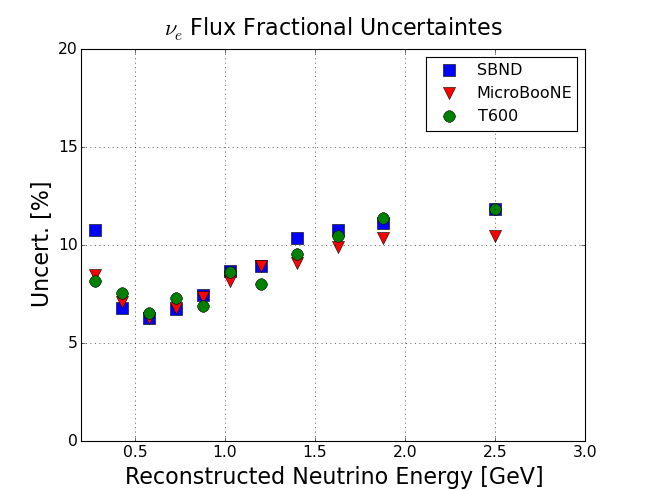
\includegraphics[width=0.5\textwidth]{systematics_figures/matrixFile_nue_ND_100m_uB_T600_onaxis_flux_6_ecalo2_nu_vePhot0.05_gap3_fracUncert}
    \caption[Fractional Flux Uncertainties]{The systematic uncertainties in the \nue appearance event rates for the SBN program, coming from uncertainties in the neutrino flux.  This includes flux-based uncertainties for both the \nue component, from the \nue flux, and the \numu misidentified component of the background.}
   \label{fig:sys_flux_uncert_fracUncert}
\end{figure}

\begin{figure}[]
    \centering
    \includegraphics[width=0.5\textwidth]{systematics_figures/matrixFile_nue_ND_100m_uB_T600_onaxis_flux_6_ecalo2_nu_vePhot0.05_gap3_fracMatHist}
    \caption[Flux Fractional Covariance Matrix]{The fractional covariance matrix for the flux uncertainties.  The uncertainties are highest in the tails of each detector's distributions.}
   \label{fig:syst_flux_fracmatrix}
\end{figure}
\begin{figure}[]
    \centering
    \includegraphics[width=0.5\textwidth]{systematics_figures/matrixFile_nue_ND_100m_uB_T600_onaxis_flux_6_ecalo2_nu_vePhot0.05_gap3_corrMatHist}
    \caption[Flux Correlation Matrix]{The correlation matrix for the flux uncertainties. The uncertainties are highly correlated across the three detectors, which is essential to achieving a strong cancellation between detectors. }
   \label{fig:syst_flux_corrmatrix}
\end{figure}



\section{Uncertainties from Neutrino Interactions}

After the flux uncertainty, the largest remaining uncertainty in a multidetector analysis is the uncertainty coming from neutrino interactions.  In particular, the flux and cross section uncertainties combine to form the overall shape uncertainty 

In a multi-detector analysis, comparisons must be performed using a shape only analysis
unless the uncertainty due to normalization is reliably quantified. For this Short Baseline
program, the neutrino interaction uncertainties (cross-section uncertainties) are the largest
uncertainties that affect the normalization of event rates at the three detectors. To study this
uncertainty, we have attempted to quantify both the absolute magnitude of uncertainty due to
cross sections as well as the correlations between detectors of these uncertainties.
The simulation used for analysis in this document were performed using the GENIE event
generator, and so all cross section uncertainties were quantified within the framework of event
reweighing that GENIE provides. In particular, we simulated 250 different “cross section uni-
verses” in which each of the parameters we intended to study was varied at random. The
variations were made to underlying physical quantities and the variations in those quantities,
though drawn at random, are consistent with a Gaussian distribution that has a 1σ spread
equal to the 1σ uncertainty in the underlying physical quantity. Much more detail is available
from the GENIE manual, chapter 8[? ], on both the underlying physical uncertainties and the
methodology for propagating them to cross section reweights.


\begin{figure}[]
    \centering
    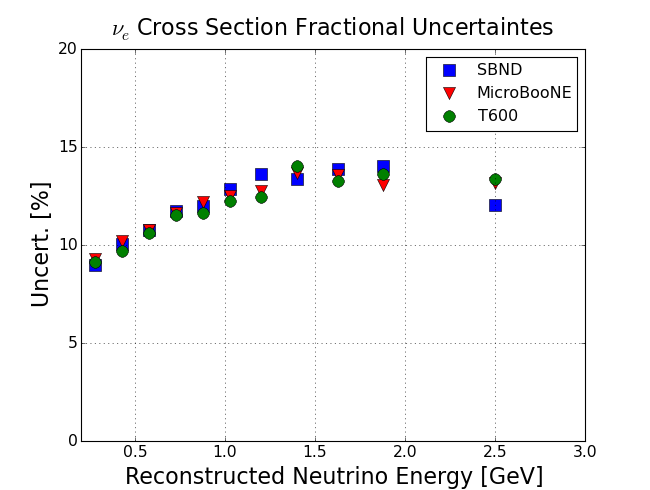
\includegraphics[width=0.5\textwidth]{systematics_figures/matrixFile_nue_ND_100m_uB_T600_onaxis_xsec_0_ecalo2_nu_vePhot0.05_gap3_fracUncert}
    \caption{}
   \label{fig:sys_xsec_uncert_fracUncert}
\end{figure}

\begin{figure}[]
    \centering
    \includegraphics[width=0.5\textwidth]{systematics_figures/matrixFile_nue_ND_100m_uB_T600_onaxis_xsec_0_ecalo2_nu_vePhot0.05_gap3_fracMatHist}
    \caption{}
   \label{fig:syst_xsec_fracmatrix}
\end{figure}
\begin{figure}[]
    \centering
    \includegraphics[width=0.5\textwidth]{systematics_figures/matrixFile_nue_ND_100m_uB_T600_onaxis_xsec_0_ecalo2_nu_vePhot0.05_gap3_corrMatHist}
    \caption{The predicted event rates for the SBN program in all three detectors, assuming 2.2e20 Protons on Target delivered each year.  For this analysis, \uboone is assumed to have 6 years of running (its original 3 + 3 with the SBN program)}.
   \label{fig:syst_xsec_corrmatrix}
\end{figure}

\section{Residual Systematic Uncertainties}

